% Source for the figure of RRRBitVector (sec. 22.5): a block of b = 8 bits
% (63 in the library) with its 1s at the places 1, 4 and 6, its class 3 and
% its offset 27 in the combinatorial number system, and the classes and the
% offsets of four blocks, of variable widths. Build: make figures.
\documentclass[border=4pt]{standalone}
\usepackage[T1]{fontenc}
\usepackage{lmodern}
\usepackage{amsmath}
\usepackage{tikz}
\usepackage{lamalunga}
% tikz-ads.tex: the TikZ styles shared by the figures of the memory of the
% manual, \input by each standalone figure: a cell of a vector (cell), the
% cell that an operation touches (touched), a free cell (free), a node of a
% linked structure (node), the labels of indices (index) and of variables
% (var), a pointer (ptr), and \cells and \indices to draw a row of cells.
\usetikzlibrary{arrows.meta,positioning,calc,fit,shapes.multipart}
\definecolor{adsTouched}{RGB}{214,196,236}
\definecolor{adsFree}{RGB}{236,236,236}
\tikzset{
  ads/.style={>={Stealth[length=2mm]},font=\small,
              every node/.append style={inner sep=0pt}},
  cell/.style={draw,minimum width=7mm,minimum height=7mm,
               font=\small\ttfamily,outer sep=0pt},
  touched/.style={cell,fill=adsTouched},
  free/.style={cell,fill=adsFree,text=black!45},
  node/.style={draw,rounded corners=1pt,minimum width=8mm,
               minimum height=6mm,font=\small\ttfamily},
  index/.style={font=\scriptsize\ttfamily,text=black!60},
  var/.style={font=\small\itshape},
  ptr/.style={->,thick}
}
% \cells{name}{x,y}{list}: a row of cells, the first at (x,y), named
% name-0, name-1, ...; each item is text/style, the style one of cell,
% touched and free (e.g., {a/cell,e/touched,/free})
\newcommand{\cells}[3]{%
  \foreach \v/\s [count=\i from 0] in {#3}
    \node[\s] (#1-\i) at ($(#2)+(\i*7mm,0)$) {\v};}
% \indices{name}{n}: the indices 0 .. n-1 under the cells of name
\newcommand{\indices}[2]{%
  \foreach \i in {0,...,\numexpr#2-1\relax}
    \node[index,below=1.2mm of #1-\i] {\i};}

\begin{document}
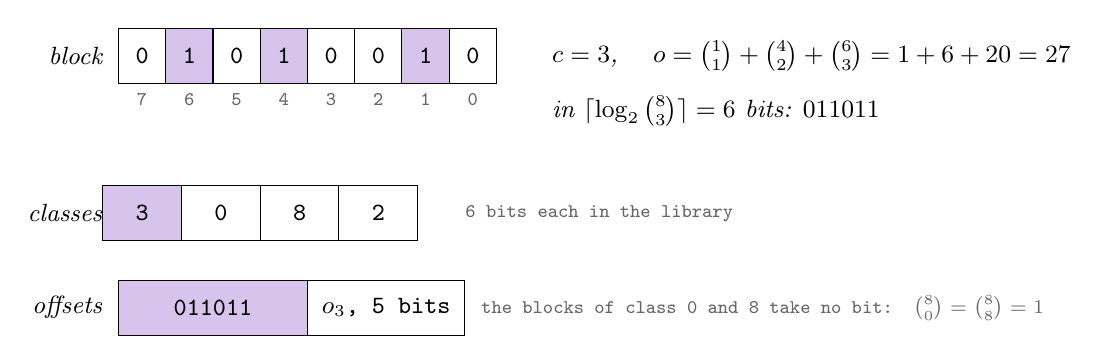
\begin{tikzpicture}[ads,bit/.style={cell,minimum width=6mm}]
  \node[var,anchor=east] at (-5mm,0) {block};
  \foreach \v/\s [count=\i from 0] in {0/cell,1/touched,0/cell,1/touched,0/cell,0/cell,1/touched,0/cell}
    \node[\s,minimum width=6mm] (x\i) at (\i*6mm,0) {\v};
  \foreach \i/\p in {0/7,1/6,2/5,3/4,4/3,5/2,6/1,7/0}
    \node[index,below=1.2mm of x\i] {\p};
  \node[var,anchor=west] at (52mm,0)
    {$c = 3$, \quad $o = \binom{1}{1} + \binom{4}{2} + \binom{6}{3} = 1 + 6 + 20 = 27$};
  \node[var,anchor=west] at (52mm,-7mm)
    {in $\lceil \log_2 \binom{8}{3} \rceil = 6$ bits: $011011$};
  % the arrays of four blocks
  \node[var,anchor=east] at (-5mm,-20mm) {classes};
  \foreach \v/\s [count=\i from 0] in {3/touched,0/cell,8/cell,2/cell}
    \node[\s,minimum width=10mm] (c\i) at (\i*10mm,-20mm) {\v};
  \node[index,anchor=west] at (41mm,-20mm) {6 bits each in the library};
  \node[var,anchor=east] at (-5mm,-32mm) {offsets};
  \node[touched,minimum width=24mm,anchor=west] (o0) at (-3mm,-32mm) {011011};
  \node[cell,minimum width=20mm,anchor=west] (o3) at (21mm,-32mm) {$o_3$, 5 bits};
  \node[index,anchor=west] at (43mm,-32mm)
    {the blocks of class 0 and 8 take no bit: $\binom{8}{0} = \binom{8}{8} = 1$};
\end{tikzpicture}
\end{document}
